\section{多元函数的极值}
\subsection{多元函数的极值及最值}
在实际问题中,往往会遇到需要求解多元函数最大值、最小值的问题.
与一元函数相类似,多元函数的最大值、最小值与极大值、极小值有密切联系.

\begin{definition}
%@see: 《高等数学(第六版 下册)》 P109 定义
%@see: 《数学分析(第二版 下册)》(陈纪修) P202 定义12.6.1
设开区域\(D \subseteq \mathbb{R}^n\),
函数\(f\colon D \to \mathbb{R}\),
点\(P_0 \in D\).
\begin{itemize}
	\item 若存在\(P_0\)的某个去心邻域\(\mathring{U}(P_0) \subseteq D\),
	使得对于任意点\(P \in \mathring{U}(P_0)\),
	都有\begin{equation*}
		f(P) < f(P_0),
	\end{equation*}
	则称“\(P_0\)是函数\(f\)的一个\DefineConcept{极大值点}”
	“\(f(P_0)\)是函数\(f\)的一个\DefineConcept{极大值}”.

	\item 若存在\(P_0\)的某个去心邻域\(\mathring{U}(P_0) \subseteq D\),
	使得对于任意点\(P \in \mathring{U}(P_0)\),
	都有\begin{equation*}
		f(P) > f(P_0),
	\end{equation*}
	则称“\(P_0\)是函数\(f\)的一个\DefineConcept{极小值点}”
	“\(f(P_0)\)是函数\(f\)的一个\DefineConcept{极小值}”.
\end{itemize}

极大值、极小值统称为\DefineConcept{极值}%
\footnote{极大值、极小值的定义不是统一的.
有的教材要求严格的序关系\(f(P) < f(P_0)\)、\(f(P) > f(P_0)\).
有的教材定义极大值、极小值时给出的不等式
分别是\(f(P) \leq f(P_0)\)、\(f(P) \geq f(P_0)\).}.
极大值点、极小值点统称为\DefineConcept{极值点}.
\end{definition}

\begin{example}%example:多元函数的极值.例1
%@see: 《高等数学(第六版 下册)》 P109 例1
函数\(z=3x^2+4y^2\)在点\((0,0)\)处有极小值
(如\cref{figure:多元函数的极值.例1}).
因为对于点\((0,0)\)的任一去心邻域内的点,函数值都为正,
而在点\((0,0)\)处函数值为零.
从几何上看这是显然的,因为点\((0,0,0)\)是开口向上的椭圆抛物面\(z=3x^2+4y^2\)的顶点.
\end{example}

\begin{figure}[htb]%z=3x^2+4y^2
	\centering
	\def\scale{.7}
	\begin{tikzpicture}[scale=\scale]
		\begin{axis}[
			xlabel=$y$,
			ylabel=$z$,
		]
			\addplot[
				surf,
				faceted color=blue,
				samples=30,
				domain=-1:1
			]{4*x^2};
		\end{axis}
	\end{tikzpicture}~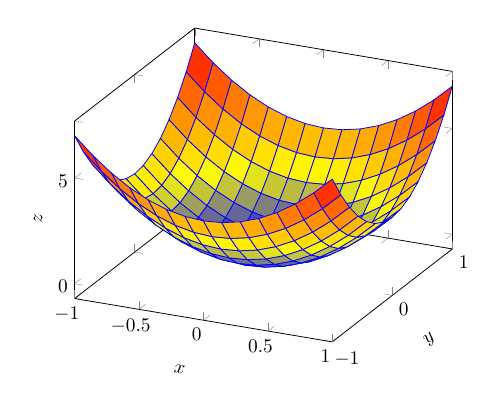
\begin{tikzpicture}[scale=\scale]
		\begin{axis}[
			xlabel=$x$,
			ylabel=$y$,
			zlabel=$z$,
			xlabel style={sloped},
			ylabel style={sloped},
		]
			\addplot3[
				surf,
				faceted color=blue,
				samples=15,
				domain=-1:1,y domain=-1:1
			]{3*x^2+4*y^2};
		\end{axis}
	\end{tikzpicture}~\begin{tikzpicture}[scale=\scale]
		\begin{axis}[
			xlabel=$x$,
			ylabel=$z$,
		]
			\addplot[
				surf,
				faceted color=blue,
				samples=30,
				domain=-1:1
			]{3*x^2};
		\end{axis}
	\end{tikzpicture}
	\caption{}%@see:[example:多元函数的极值.例1]
	\label{figure:多元函数的极值.例1}
\end{figure}

\subsection{多元函数极值存在的条件}
二元函数的极值问题,一般可以利用偏导数来解决.
下面两个定理就是关于这个问题的结论.
\begin{theorem}[必要条件]\label{theorem:多元函数微分法.多元函数极值存在的必要条件}
%@see: 《高等数学(第六版 下册)》 P110 定理1(必要条件)
%@see: 《数学分析(第二版 下册)》(陈纪修) P202 定理12.6.1(必要条件)
设函数\(z=f(x,y)\)在点\(P_0(x_0,y_0)\)具有偏导数,且在点\(P_0\)处有极值,则有\begin{equation*}
	f'_x(x_0,y_0) = f'_y(x_0,y_0) = 0.
\end{equation*}
\begin{proof}
不妨设\(z=f(x,y)\)在点\((x_0,y_0)\)处有极大值.
根据定义,
在点\((x_0,y_0)\)的某去心邻域内的点\((x,y)\)都满足不等式\begin{equation*}
	f(x,y)<f(x_0,y_0).
\end{equation*}
特别地,在该邻域内取\(y=y_0\)而\(x\neq x_0\)的点,也应满足不等式\begin{equation*}
	f(x,y_0)<f(x_0,y_0).
\end{equation*}
这表明一元函数\(f(x,y_0)\)在\(x=x_0\)处取得极大值,
因而必有\begin{equation*}
	f'_x(x_0,y_0)=0.
\end{equation*}

类似地可证\begin{equation*}
	f'_y(x_0,y_0)=0.
\end{equation*}
\end{proof}
\end{theorem}

从几何上看,这时如果曲面\(z=f(x,y)\)在点\((x_0,y_0,z_0)\ (z_0=f(x_0,y_0))\)处有切平面,
则切平面\begin{equation*}
	z-z_0=f'_x(x_0,y_0)(x-x_0)+f'_y(x_0,y_0)(y-y_0)
\end{equation*}成为平行于\(xOy\)坐标面的平面\(z=z_0\).

仿照一元函数,我们给出多元函数的“驻点”的定义.
\begin{definition}
%@see: 《高等数学(第六版 下册)》 P110
%@see: 《数学分析(第二版 下册)》(陈纪修) P203
使函数的梯度为零的点
称为“函数\(f\)的\DefineConcept{驻点}”.
\end{definition}
那么\cref{theorem:多元函数微分法.多元函数极值存在的必要条件}
可以说成“具有偏导数的函数的极值点必定是驻点,但函数的驻点不一定是极值点”.
例如,点\((0,0)\)是函数\(f(x,y) = xy\)的驻点,但函数\(f\)在该点并无极值.

\begin{theorem}[充分条件]\label{theorem:多元函数微分法.多元函数极值存在的充分条件}
%@see: 《高等数学(第六版 下册)》 P110 定理2(充分条件)
%@see: 《数学分析(第二版 下册)》(陈纪修) P205 定理12.6.2
设\((x_0,y_0)\)是函数\(f\colon \mathbb{R}^2 \supseteq D \to \mathbb{R}\)的驻点,
且\(f\)在点\((x_0,y_0)\)的某一邻域内具有二阶连续偏导数,
令\begin{equation*}
	A \defeq f''_{xx}(x_0,y_0),
	\quad
	B \defeq f''_{xy}(x_0,y_0),
	\quad
	C \defeq f''_{yy}(x_0,y_0),
\end{equation*}
则\(f(x,y)\)在\((x_0,y_0)\)处是否取得极值的条件如下:
\begin{itemize}
	\item \(AC-B^2>0\)时具有极值,
	当\(A<0\)时\(f(x_0,y_0)\)是极大值,
	当\(A>0\)时\(f(x_0,y_0)\)是极小值.
	\item \(AC-B^2<0\)时没有极值.
	\item \(AC-B^2=0\)时可能有极值,也可能没有极值.
\end{itemize}
%TODO proof
\end{theorem}

\begin{example}
当\(AC-B^2=0\)时,函数可能有极值,也可能没有极值;
即便函数有极值,可能是极大值,也可能是极小值.
对于以下三个函数\begin{equation*}
	f(x,y) = x^2 y^2,
	\qquad
	g(x,y) = -x^2 y^2,
	\qquad
	h(x,y) = x^2 y^3,
\end{equation*}
它们在原点\((0,0)\)处都有\(AC-B^2=0\),
但是\(f\)在原点取极小值,\(g\)在原点取极大值,而\(h\)在原点没有极值.
\end{example}

\begin{example}
求函数\(f(x,y) = x^3-y^3+3x^2+3y^2-9x\)的极值.
\begin{solution}
先解方程组\begin{equation*}
	\left\{ \begin{array}{l}
		f'_x(x,y) = 3x^2+6x-9 = 0, \\
		f'_y(x,y) = -3y^2+6y = 0,
	\end{array} \right.
\end{equation*}
求得驻点为\((1,0),(1,2),(-3,0),(-3,2)\).

再求出二阶偏导数\begin{equation*}
	f''_{xx}(x,y) = 6x+6,
	\qquad
	f''_{xy}(x,y) = 0,
	\qquad
	f''_{yy}(x,y) = -6y+6.
\end{equation*}

在点\((1,0)\)处,\(AC-B^2=12\cdot6>0\),又\(A=12>0\),
所以函数在\((1,0)\)处有极小值\(f(1,0)=-5\);
在点\((1,2)\)处,\(AC-B^2=12\cdot(-6)<0\),
所以点\((1,2)\)不是极值点;
在点\((-3,0)\)处,\(AC-B^2=(-12)\cdot6<0\),
所以点\((-3,0)\)不是极值点;
在点\((-3,2)\)处,\(AC-B^2=(-12)\cdot(-6)>0\),又\(A=-12<0\),
所以函数在\((-3,2)\)处有极大值\(f(-3,2)=31\).
\end{solution}
\end{example}

\begin{example}
求函数\(f(x,y) = (y-x^2)(y-x^3)\)的极值.
\begin{solution}
对\(f(x,y) = y^2 - (x^2+x^3) y + x^5\)求偏导,得\begin{equation*}
	f'_x = 5x^4 - y(2x+3x^2),
	\qquad
	f'_y = 2y - x^2 - x^3.
\end{equation*}

令\(f'_x = f'_y = 0\).
当\(x=0\)时,解得\(y = 0\);
当\(x\neq0\)时,有\begin{equation*}
	\begin{cases}
		5x^4-y(2x+3x^2) = 0, \\
		2y-x^2+x^3 = 0,
	\end{cases}
\end{equation*}
于是\begin{equation*}
	5x^4 = \frac{x^2+x^3}{2}(2x+3x^2),
\end{equation*}
整理得\begin{equation*}
	3x^5-5x^4+2x^3=0,
\end{equation*}
即\begin{equation*}
	3x^2-5x+2=0,
\end{equation*}
解得\(x=1,y=1\)或\(x=2/3,y=10/27\).
也就是说,函数\(f\)的驻点为\begin{equation*}
	(0,0), \qquad
	(1,1), \qquad
	(2/3,10/27).
\end{equation*}

再对\(f\)求二阶偏导,得\begin{equation*}
	f''_{xx} = 20x^3 - y(2+6x),
	\qquad
	f''_{xy} = -2x-3x^2,
	\qquad
	f''_{yy} = 2.
\end{equation*}
那么
\begin{equation*}
	f''_{xx}(0,0) = 0,
	\qquad
	f''_{xy}(0,0) = 0,
	\qquad
	f''_{yy}(0,0) = 2,
\end{equation*}\begin{equation*}
	f''_{xx}(1,1) = 12,
	\qquad
	f''_{xy}(1,1) = -5,
	\qquad
	f''_{yy}(1,1) = 2,
\end{equation*}\begin{equation*}
	f''_{xx}(2/3,10/27) = 100/27,
	\qquad
	f''_{xy}(2/3,10/27) = -8/3,
	\qquad
	f''_{yy}(2/3,10/27) = 2.
\end{equation*}

在点\((0,0)\)处\(AC-B^2 = 0\);
取\(k>0\),由于\begin{equation*}
f(-k,0) = -k^5 < f(0,0) = 0 < f(k,0) = k^5,
\end{equation*}所以函数\(f\)在点\((0,0)\)处不存在极值.

在点\((1,1)\)处\(AC-B^2 < 0\),
所以函数\(f\)在点\((1,1)\)处也没有极值.

在点\((2/3,10/27)\)处\(AC-B^2 > 0\)且\(A>0\),
所以函数\(f\)在点\((2/3,10/27)\)处存在极小值\begin{equation*}
	f(2/3,10/27) = -4/729.
\end{equation*}
\end{solution}
\end{example}

我们进一步推广到\(n\)元函数上.
\begingroup
\def\x{\vb{X}}
\def\X#1{\x_{#1}}
\def\z{\vb{0}}

\begin{theorem}\label{theorem:多元函数微分法.n元函数极值存在的条件}
%@see: 《线性代数》(张慎语、周厚隆) P135 定理7
%@see: 《数学分析(第二版 下册)》(陈纪修) P206 定理12.6.3
设函数\(y = f(\AutoTuple{x}{n})\)
在点\(\X0=(\AutoTuple{\xi}{n})^T\in\mathbb{R}^n\)的邻域内
存在一阶连续偏导数\begin{equation*}
	f'_i = \pdv{f}{x_i}
	\quad(i=1,2,\dotsc,n)
\end{equation*}
和二阶连续偏导数\begin{equation*}
	f''_{ij} = \pdv[2]{f}{x_i}{x_j}
	\quad(i,j=1,2,\dotsc,n).
\end{equation*}
记\(f\)的梯度为\(\grad f(\x)
= \left(\pdv{f}{x_1},\pdv{f}{x_2},\dotsc,\pdv{f}{x_n}\right)^T\),
\(f\)的黑森矩阵为\(\hessian f = (f''_{ij})_n\),
则\begin{itemize}
	\item 当\(\grad f(\X0) = \z\),且\(\hessian f\)正定时,
	\(f(\x)\)在\(\X0\)处取得极小值;
	\item 当\(\grad f(\X0) = \z\),且\(\hessian f\)负定时,
	\(f(\x)\)在\(\X0\)处取得极大值;
	\item 当\(\grad f(\X0) = \z\),且\(\hessian f\)半正定或半负定时,
	\(f(\x)\)可能有极值,也可能没有极值\footnote{%
	这时候需要考察更高阶偏导数,才能确定函数的极值是否存在,是极大值还是极小值.};
	\item 当\(\grad f(\X0) = \z\),且\(\hessian f\)不定时,
	\(\X0\)不是\(f(\x)\)的极值点.
\end{itemize}
\begin{proof}
将\(y = f(\x)\)在\(\X0\)处作泰勒展开,得\begin{equation*}
	f(\x) = f(\X0)
	+ \sum_{i=1}^n f'_i(\X0) h_i
	+ \frac{1}{2} \sum_{i=1}^n \sum_{j=1}^n
		f''_{ij}(\X0+\theta\increment\x) h_i h_j,
\end{equation*}
其中\(\increment\x=\x-\X0=(h_1,h_2,\dotsc,h_n)^T,
h_i = x_i - \xi_i\ (i=1,2,\dotsc,n),
0<\theta<1\).

由于\(\grad f(\X0) = \z\)且\(f(\x)\)的所有二阶偏导数连续,
故\(\sum_{i=1}^n f'_i(\X0) h_i = 0\),
\begin{align*}
	f(\x) - f(\X0)
	&= \frac{1}{2} \sum_{i=1}^n \sum_{j=1}^n
		f''_{ij}(\X0+\theta\increment\x) h_i h_j \\
	&= \frac{1}{2} \sum_{i=1}^n \sum_{j=1}^n
		f''_{ij}(\X0) h_i h_j
		+ \frac{1}{2} \sum_{i=1}^n \sum_{j=1}^n
		\epsilon_{ij} h_i h_j \\
	&= \frac{1}{2} (\increment\x)^T [\hessian f + (\epsilon_{ij})_n] (\increment\x),
\end{align*}
其中\(\epsilon_{ij} = f''_{ij}(\X0+\theta\increment\x) - f''_{ij}(\X0)\),
且\begin{equation*}
	\epsilon_{ij} = \epsilon_{ji}\to0\ (\increment\x\to\z)
	\quad(i,j=1,2,\dotsc,n).
\end{equation*}

当实对称矩阵\(\hessian f\)正定时,其各阶顺序主子式全大于零,
那么根据行列式的定义和极限的保号性,当\(\abs{\increment\x}\to0\)时,
\(\hessian f + (\epsilon_{ij})_n\)的各阶顺序主子式也全大于零,
故\(\hessian f + (\epsilon_{ij})_n\)依然正定,便得\(f(\x) - f(\X0) > 0\),
也就是说\(f(\x)\)在\(\X0\)取到极大值\(f(\X0)\).

同理可证其他两种情形下的结论.
\end{proof}
\end{theorem}

\begin{example}
%@see: 《线性代数》(张慎语、周厚隆) P136 例1
求函数\(f(x,y) = 2x^2 + xy + y^2 + ax - 5y\)的极值.
\begin{solution}
显然,函数\(f\)的各阶偏导数都连续.
令\begin{equation*}
	\grad f(x,y) = \begin{bmatrix} f'_x \\ f'_y \end{bmatrix}
	= \begin{bmatrix} 4x+y+a \\ x+2y-5 \end{bmatrix} = \z,
\end{equation*}
解得驻点为\(\X0 = \frac{1}{7} \begin{bmatrix} -5-2a \\ 20+a \end{bmatrix}\).

\(\hessian f = \begin{bmatrix}
	f''_{11} & f''_{12} \\
	f''_{21} & f''_{22}
\end{bmatrix}
= \begin{bmatrix}
4 & 1 \\
1 & 2
\end{bmatrix}\)是正定矩阵,
故\(f\)在\(\X0\)处取得极小值\(\frac{1}{7} (-50-5a-a^2)\).
\end{solution}
\end{example}

\begin{proposition}
%@see: 《线性代数》(张慎语、周厚隆) P135 例2
设\(\vb{A} = (a_{ij})_n\)是\(n\)阶实对称正(负)定矩阵,
则\(n\)元实二次函数\begin{equation*}
	f(\AutoTuple{x}{n})
	= \sum_{i=1}^n \sum_{j=1}^n a_{ij} x_i x_j
	+ 2 \sum_{i=1}^n b_i x_i + c
\end{equation*}有唯一的极小(大)值.
\begin{proof}
设\(\vb{X} = (\AutoTuple{x}{n})^T,
\vb{B} = (\AutoTuple{b}{n})^T\),
则一阶偏导数\begin{equation*}
	f'_i(\vb{X})
	= 2 \sum_{j=1}^n a_{ij} x_j + 2 b_j
	\quad(i=1,2,\dotsc,n)
\end{equation*}和二阶偏导数\begin{equation*}
	f''_{ij}(\vb{X})
	= 2 a_{ij}
	\quad(i,j=1,2,\dotsc,n)
\end{equation*}连续,
令\begin{equation*}
	\grad f
	= 2 \vb{A} \vb{X} + 2 \vb{B}
	= \vb0,
\end{equation*}
由于\(\vb{A}\)正(负)定,故\(\vb{A}\)可逆,
从而可以解出唯一驻点\(\vb{X}_0 = -\vb{A}^{-1} \vb{B}\).
又因为\(\hessian f
= 2 \vb{A}\)也正(负)定,
故\(f(\AutoTuple{x}{n})\)
在\(\vb{X}_0 = -\vb{A}^{-1} \vb{B}\)
取得唯一的极小(大)值:\begin{equation*}
	\vb{X}_0^T \vb{A} \vb{X}_0
	+ 2 \vb{X}_0^T \vb{B} + c
	= \vb{X}_0^T (\vb{A} \vb{X}_0 + \vb{B})
	+ \vb{X}_0^T \vb{B} + c
	= -\vb{B}^T \vb{A}^{-1} \vb{B} + c.
\end{equation*}
\end{proof}
\end{proposition}

\subsection{极值点的求解思路}
利用\cref{theorem:多元函数微分法.多元函数极值存在的必要条件,%
theorem:多元函数微分法.多元函数极值存在的充分条件,%
theorem:多元函数微分法.n元函数极值存在的条件},
我们把具有二阶连续偏导数的函数\(z = f(x,y)\)的极值的求法叙述如下:
\begin{enumerate}
	\item 解方程组\begin{equation*}
		f'_x(x,y) = 0
		\quad\text{和}\quad
		f'_y(x,y) = 0,
	\end{equation*}求得一切实数解,即可求得一切驻点.

	\item 对于每一个驻点\((x_0,y_0)\),
	求出二阶偏导数的值\(A=f''_{xx}\)、\(B=f''_{xy}\)和\(C=f''_{yy}\).

	\item 定出\(AC-B^2\)的符号,
	按\cref{theorem:多元函数微分法.多元函数极值存在的充分条件}
	的结论判定\(f(x_0,y_0)\)是不是极值,是极大值还是极小值.
	当\(AC-B^2=0\)时,可以借助极值的定义判断是否存在极值以及极值的类型.
\end{enumerate}

讨论函数的极值问题时,如果函数在所讨论的区域内具有偏导数,则极值只可能在驻点处取得.
然而,如果函数在个别点处的偏导数不存在,这些点当然不是驻点,但也可能是极值点.
例如,函数\(f(x,y) = -\sqrt{x^2+y^2}\)在点\((0,0)\)处的偏导数不存在,
但该函数在点\((0,0)\)处却具有极大值.
因此,在考虑函数的极值问题时,除了考虑函数的驻点外,
如果有偏导数不存在的点,那么对这些点也应当考虑.

\subsection{最值点的求解思路}
与一元函数相类似,我们可以利用函数的极值来求函数的最值.
我们知道,如果\(f(x,y)\)在有界闭区域\(D\)上连续,
则\(f(x,y)\)在\(D\)上必定能取得最大值和最小值.
这种使函数取得最大值或最小值的点(即最值点)既可能在\(D\)的内部,也可能在\(D\)的边界上.
我们假定,函数在\(D\)上连续,在\(D\)内可微分且只有有限个驻点,
这时如果函数在\(D\)的内部取得最大值(或最小值),则这个最值也是函数的极值.
因此,这上述假定下,求函数的最值的一般方法是:
将函数\(f(x,y)\)在\(D\)内的所有驻点处的函数值及在\(D\)的边界上的最值相互比较,
其中最大的就是最大值,最小的就是最小值.
但这种做法,由于要求出\(f(x,y)\)在\(D\)的边界上的最值,所以往往相当复杂.
在通常遇到的实际问题中,如果根据问题的性质,
知道函数\(f(x,y)\)的最值一定在\(D\)的内部取得,
而函数在\(D\)内只有一个驻点,
那么可以肯定该驻点处的函数值就是函数\(f(x,y)\)在\(D\)上的最值.

\subsection{拉格朗日乘数法 --- 条件极值的求解思路}\label{section:多元函数微分法.拉格朗日乘数法}
上面所讨论的极值问题,对于函数的自变量,除了限制在函数的定义域内以外,
并无其他条件,所以有时候称为\DefineConcept{无条件极值}.
但在实际问题中,有时会遇到对函数的自变量还有约束条件的极值问题.
例如,求表面积为\(a^2\)而体积为最大的长方体的体积问题.
设长方体的三棱的长为\(x,y,z\),则体积为\(V = xyz\).
又因假定表面积为\(a^2\),所以自变量\(x,y,z\)还必须满足约束条件\(2(xy+yz+zx)=a^2\).
像这种对自变量有约束条件的极值称为\DefineConcept{条件极值}.
对于有些实际问题,可以把条件极值化为无条件极值,然后利用前面的方法加以解决.
例如上述问题,可由条件\(2(xy+yz+zx)=a^2\),将\(z\)表成\(x,y\)的函数\begin{equation*}
	z = \frac{a^2-2xy}{2(x+y)}.
\end{equation*}
再把它代入\(V = xyz\)中,于是问题就化为求\begin{equation*}
	V = \frac{xy}{2} \frac{a^2-2xy}{x+y}
\end{equation*}的无条件极值.

但在很多情形下,将条件极值化为无条件极值并不这样简单.
另有一种直接寻求条件极值的方法,可以不必先把问题化到无条件极值的问题,
这就是下面要介绍的\DefineConcept{拉格朗日乘数法}(Lagrange multiplier).
%@see: https://mathworld.wolfram.com/LagrangeMultiplier.html
%@see: https://tutorial.math.lamar.edu/classes/calciii/lagrangemultipliers.aspx

我们先寻求函数
\begin{equation}\label{equation:拉格朗日乘数法.目标函数1}
%@see: 《高等数学(第六版 下册)》 P114 公式(1)
	z=f(x,y)
\end{equation}
在条件
\begin{equation}\label{equation:拉格朗日乘数法.限制条件1}
%@see: 《高等数学(第六版 下册)》 P114 公式(2)
	\phi(x,y)=0
\end{equation}
下取得极值的必要条件.

如果函数 \labelcref{equation:拉格朗日乘数法.目标函数1}
在\(P_0(x_0,y_0)\)取得所求的极值,
那么首先有
\begin{equation}\label{equation:拉格朗日乘数法.限制条件1在P0}
%@see: 《高等数学(第六版 下册)》 P114 公式(3)
	\phi(x_0,y_0)=0.
\end{equation}
我们假定在\((x_0,y_0)\)的某一邻域内
\(f(x,y)\)与\(\phi(x,y)\)均有连续的一阶偏导数,
而\(\phi'_y(x_0,y_0)\neq0\).
由隐函数存在定理可知,
方程 \labelcref{equation:拉格朗日乘数法.限制条件1}
确定一个连续且具有连续导数的函数\(y=\psi(x)\),
将其代入\cref{equation:拉格朗日乘数法.目标函数1},
结果得到一个变量\(x\)的函数
\begin{equation}\label{equation:拉格朗日乘数法.目标函数1.代入限制条件1}
%@see: 《高等数学(第六版 下册)》 P114 公式(4)
	z=f(x,\psi(x)).
\end{equation}
于是函数 \labelcref{equation:拉格朗日乘数法.目标函数1} 在\((x_0,y_0)\)取得所求的极值,
也就是相当于函数 \labelcref{equation:拉格朗日乘数法.目标函数1.代入限制条件1} 在\(x=x_0\)取得极值.
由一元可导函数取得极值的必要条件知道
\begin{equation}\label{equation:拉格朗日乘数法.目标函数1取得极值的必要条件1}
%@see: 《高等数学(第六版 下册)》 P114 公式(5)
	\dv{z}{x}\eval_{x=x_0}
	= f'_x(x_0,y_0) + f'_y(x_0,y_0) \dv{y}{x}\eval_{x=x_0}
	= 0,
\end{equation}
而由\cref{equation:拉格朗日乘数法.限制条件1} 用隐函数求导公式,有\begin{equation*}
	\dv{y}{x}\eval_{x=x_0}
	= -\frac{\phi'_x(x_0,y_0)}{\phi'_y(x_0,y_0)}.
\end{equation*}
把上式代入\cref{equation:拉格朗日乘数法.目标函数1取得极值的必要条件1},得
\begin{equation}\label{equation:拉格朗日乘数法.目标函数1取得极值的必要条件2}
%@see: 《高等数学(第六版 下册)》 P114 公式(6)
	f'_x(x_0,y_0) - f'_y(x_0,y_0) \frac{\phi'_x(x_0,y_0)}{\phi'_y(x_0,y_0)}
	= 0.
\end{equation}
\labelcref{equation:拉格朗日乘数法.限制条件1在P0,equation:拉格朗日乘数法.目标函数1取得极值的必要条件2}
两式就是函数 \labelcref{equation:拉格朗日乘数法.目标函数1}
在条件 \labelcref{equation:拉格朗日乘数法.限制条件1} 下
在\((x_0,y_0)\)取得极值的必要条件.

令\(\lambda=-\frac{f'_y(x_0,y_0)}{\phi'_y(x_0,y_0)}\),
则上述必要条件就变为
\begin{equation}\label{equation:拉格朗日乘数法.目标函数1取得极值的必要条件3}
	\left\{ \begin{array}{l}
		f'_x(x_0,y_0) + \lambda \phi'_x(x_0,y_0) = 0, \\
		f'_y(x_0,y_0) + \lambda \phi'_y(x_0,y_0) = 0, \\
		\phi(x_0,y_0) = 0.
	\end{array} \right.
\end{equation}

若引进辅助函数\begin{equation*}
	L(x,y) = f(x,y) + \lambda \phi(x,y),
\end{equation*}
则不难看出,
\cref{equation:拉格朗日乘数法.目标函数1取得极值的必要条件3} 中前两式就是\begin{equation*}
	L'_x(x_0,y_0)=0, \qquad
	L'_y(x_0,y_0)=0.
\end{equation*}
我们把函数\(L(x,y)\)称为\DefineConcept{拉格朗日函数},
把参数\(\lambda\)称为\DefineConcept{拉格朗日乘子}.

由以上讨论,我们得到以下结论.

要找函数\(z=f(x,y)\)在约束条件\(\phi(x,y)=0\)下的可能极值点,
可以先作拉格朗日函数\begin{equation*}
	L(x,y) = f(x,y) + \lambda \phi(x,y),
\end{equation*}
其中\(\lambda\)为参数.
求其对\(x\)与\(y\)的一阶偏导数,并使之为零,
然后与限定条件方程联立起来:\begin{equation*}
	\left\{ \begin{array}{l}
		f'_x(x,y)+\lambda\phi'_x(x,y)=0, \\
		f'_y(x,y)+\lambda\phi'_y(x,y)=0, \\
		\phi(x,y)=0.
	\end{array} \right.
\end{equation*}
由这方程组解出\(x,y,\lambda\),
这样得到的\((x,y)\)就是函数\(f(x,y)\)在附件条件\(\phi(x,y)=0\)下的可能极值点.

%@see: 《数学分析(第二版 下册)》(陈纪修) P221 定理12.7.1(条件极值的必要条件)
这方法还可以推广到自变量多于两个而条件多于一个的情形.
例如,要求目标函数\begin{equation*}
	f\colon \mathbb{R}^n \to \mathbb{R}, P = (\AutoTuple{x}{n})^T \mapsto u
\end{equation*}在\(m\ (m<n)\)个约束条件\begin{equation*}
	\phi_i(P) = 0
	\quad(i=1,2,\dotsc,m)
\end{equation*}下的极值,
这里\(f,\phi_i\ (i=1,2,\dotsc,m)\)都具有连续偏导数,
且雅克比矩阵\begin{equation*}
	\vb{J} = \jacobi{\AutoTuple{\phi}{m}}{\AutoTuple{x}{n}}
\end{equation*}在满足约束条件的点处是满秩的,即\(\rank\vb{J} = m\).
可以证明:只要点\(P_0\)是函数\(f\)满足约束条件的条件极值点,
则必存在\(m\)个常数\(\AutoTuple{\lambda}{n}\),
使得在点\(P_0\)成立\begin{equation}
	\grad f = \sum_{k=1}^m \lambda_k \grad \phi_k.
\end{equation}
因此,我们还是可以先构造拉格朗日函数\begin{equation}
	L(P) = f(P) + \sum_{i=1}^m \lambda_i \phi_i(P),
\end{equation}
其中\(\lambda_k\ (k=1,2,\dotsc,m)\)均为参数.
求其一阶偏导数,并使之为零,然后与条件方程组联立起来求解,
即\begin{equation}\label{equation:拉格朗日乘数法.可能极值点方程}
	\left\{ \def\arraystretch{1.5} \begin{array}{ll}
		L'_i(P) = 0 & (i=1,2,\dotsc,n), \\
		\phi_j(P) = 0 & (j=1,2,\dotsc,m).
	\end{array} \right.
\end{equation}
其中\(L'_i = \pdv{L}{x_i}\).
这样得出的点\(P\)就是函数\(f(P)\)在约束条件方程组下的可能极值点.

虽然我们可以根据
%@see: 《数学分析(第二版 下册)》(陈纪修) P221 定理12.7.2
拉格朗日函数\(L\)
在满足方程组 \labelcref{equation:拉格朗日乘数法.可能极值点方程} 的点\(P_0\)的
黑森矩阵\(\hessian L(P_0)\)的性质判断极值点的类型(
若\(\hessian L(P_0)\)是正定矩阵,则\(P_0\)是条件极小值点;
若\(\hessian L(P_0)\)是负定矩阵,则\(P_0\)是条件极大指点),
但是在实际问题中,往往可根据问题本身的性质来判定.

\begin{example}
%@see: 《高等数学(第六版 下册)》 P116 例7
求表面积为\(a^2\)而体积为最大的长方体的体积.
\begin{solution}
设长方体的三棱长为\(x,y,z\),
则问题就是在条件\begin{equation*}
	\phi(x,y,z) = 2xy+2yz+2zx-a^2 = 0
	\eqno(1)
\end{equation*}下,
求函数\begin{equation*}
	V = xyz
	\quad (x>0,y>0,z>0)
	\eqno(2)
\end{equation*}的最大值.
作拉格朗日函数\begin{equation*}
	L(x,y,z) = xyz + \lambda(2xy+2yz+2zx-a^2),
\end{equation*}
求其对\(x,y,z\)的偏导数,并使之为零,得到\begin{equation*}
	\left\{ \begin{array}{l}
		yz+2\lambda(y+z) = 0, \\
		xz+2\lambda(x+z) = 0, \\
		xy+2\lambda(y+x) = 0.
	\end{array} \right.
	\eqno(3)
\end{equation*}
因\(x,y,z\)都不等于零,所以由(3)式可得\begin{equation*}
	\frac{x}{y} = \frac{x+z}{y+z},
	\qquad
	\frac{y}{z} = \frac{x+y}{x+z}.
\end{equation*}
由以上两式解得\begin{equation*}
x=y=z.
\end{equation*}
将此代入(1)式,得\begin{equation*}
	x = y = z = \frac{\sqrt{6}}{6} a,
\end{equation*}
这是唯一可能的极值点.
因为由问题本身可知最大值一定存在,所以最大值就在这个可能的极值点处取得.
也就是说,表面积为\(a^2\)的长方体中,
以棱长为\(\frac{\sqrt{6}}{6}a\)的正方体的体积为最大,
最大体积\(V = \frac{\sqrt{6}}{36} a^3\).
\end{solution}
\end{example}
\begin{example}
%@see: 《高等数学(第六版 下册)》 P119 习题9-8 10.
求内接于半径为\(a\)的球且有最大体积的长方体.
\begin{solution}
设长方体的三棱的长为\(2x,2y,2z\),
则问题就是在条件\begin{equation*}
	x^2+y^2+z^2 = a^2
\end{equation*}下,
求函数\begin{equation*}
	V = 8xyz
	\quad (x>0,y>0,z>0)
\end{equation*}的最大值.
作拉格朗日函数\begin{equation*}
	L(x,y,z,\lambda)
	= xyz + \lambda(x^2+y^2+z^2-a^2).
\end{equation*}
令\begin{gather*}
	L'_x = yz + 2\lambda x = 0, \tag1 \\
	L'_y = xz + 2\lambda y = 0, \tag2 \\
	L'_z = xy + 2\lambda z = 0, \tag3 \\
	L'_\lambda = x^2+y^2+z^2-a^2 = 0. \tag4
\end{gather*}
由(1)(2)(3)三式可得\(x = y = z\),
再代入(4)式,得\(3 x^2 = a^2\),
故\begin{equation*}
	x = y = z = \frac1{\sqrt3} a.
\end{equation*}
因此三棱长同为\(\frac2{\sqrt3} a\)的正方体的体积为最大,
体积为\(\frac8{3\sqrt3} a^3\).
\end{solution}
\end{example}
\begin{example}
%@see: 《高等数学(第六版 下册)》 P119 习题9-8 11.
设旋转抛物面\(z = x^2 + y^2\)被平面\(x + y + z = 1\)截成一个椭圆\(C\).
求椭圆\(C\)上的点到原点的距离的最大值与最小值.
\begin{solution}
所求问题就是在条件\begin{equation*}
	z = x^2 + y^2,
	\qquad
	x + y + z = 1
\end{equation*}下,
求函数\begin{equation*}
	r = \sqrt{x^2+y^2+z^2}
\end{equation*}的最值.
作拉格朗日函数\begin{equation*}
	L(x,y,z,\lambda,\mu)
	= x^2+y^2+z^2 + \lambda(x^2+y^2-z) + \mu(x+y+z-1).
\end{equation*}
令\begin{gather*}
	L'_x = 2x + 2\lambda x + \mu = 0, \tag1 \\
	L'_y = 2y + 2\lambda y + \mu = 0, \tag2 \\
	L'_z = 2z - \lambda + \mu = 0, \tag3 \\
	L'_\lambda = x^2+y^2-z = 0, \tag4 \\
	L'_\mu = x+y+z-1 = 0. \tag5
\end{gather*}
由(1)(2)两式可知\(x = y\),
再代入(4)(5)两式可知\begin{equation*}
	x = y = -\frac12 \pm \frac{\sqrt3}2,
	\qquad
	z = 1-2x = 2 \mp \sqrt3.
\end{equation*}
那么\begin{equation*}
	r = \sqrt{x^2+y^2+z^2}
	= \sqrt{9 \mp 5\sqrt3}.
\end{equation*}
于是椭圆\(C\)上的点到原点的距离的
最大值是\(\sqrt{9+5\sqrt3}\),
最小值是\(\sqrt{9-5\sqrt3}\).
\end{solution}
\end{example}

\begin{example}
%@see: 《高等数学(第六版 下册)》 P116 例8
求函数\(u=xyz\)在约束条件\begin{equation*}
	\frac{1}{x}+\frac{1}{y}+\frac{1}{z}=\frac{1}{a}
	\quad(x>0,y>0,z>0,a>0)
\end{equation*}下的极值.
\begin{solution}
作拉格朗日函数\begin{equation*}
	L(x,y,z) = xyz+\lambda\left(\frac{1}{x}+\frac{1}{y}+\frac{1}{z}-\frac{1}{a}\right).
\end{equation*}
令\begin{equation*}
	L'_x = yz - \frac{\lambda}{x^2} = 0,
	\qquad
	L'_y = xz - \frac{\lambda}{y^2} = 0,
	\qquad
	L'_z = xy - \frac{\lambda}{z^2} = 0.
\end{equation*}
注意到以上三个方程左端的第一项都是三个变量\(x,y,z\)中某两个变量的乘积,
将各方程两端同乘以相应缺少的那个变量,使得各方程左端的第一项都成为\(xyz\),
然后将所得的三个方程左、右两端相加,得\begin{equation*}
	3xyz - \lambda\left(\frac{1}{x}+\frac{1}{y}+\frac{1}{z}\right) = 0,
\end{equation*}
代入约束条件,得\begin{equation*}
	xyz = \frac{\lambda}{3a}.
\end{equation*}
再把这个结果分别代入偏微分方程组,便得\(x = y = z = 3a\).
由此得到点\((3a,3a,3a)\)是函数\(u = xyz\)在给定的约束条件下唯一可能的极值点.

把约束条件确定的隐函数记作\(v = z(x,y)\),将目标函数看作\(u = xyv = F(x,y)\),\begin{equation*}
\pdv{F}{x} = y\left(v+x\pdv{v}{x}\right);
\end{equation*}再运用\cref{theorem:多元函数微分法.多元函数极值存在的充分条件} 判断,
可知点\((3a,3a,3a)\)是函数\(u = xyz\)在给定约束条件下的极小值点,
函数\(u = xyz\)在该点处取得极小值\(27a^3\).
\end{solution}
\end{example}

\begin{example}
%@see: 《高等数学(第六版 下册)》 P117 例9
设某电视机厂生产一台电视机的成本为\(c\),
每台电视机的销售价格为\(p\),销售量为\(x\).
假设该厂的生产处于平衡状态,即电视机的生产量等于销售量.
根据市场预测,销售量\(x\)与销售价格\(p\)之间有下面的关系:\begin{equation*}
%@see: 《高等数学(第六版 下册)》 P117 (14)
	x = M e^{-ap}
	\quad(M>0,a>0),
\end{equation*}
其中\(M\)是市场最大需求量,\(a\)是价格系数.
同时,生产部门根据对生产环节的分析,对每台电视机的生产成本\(c\)有如下测算:\begin{equation*}
%@see: 《高等数学(第六版 下册)》 P117 (15)
	c = c_0 - k \ln x
	\quad(k>0,x>1),
\end{equation*}
其中\(c_0\)是只生产一台电视机时的成本,\(k\)是规模系数.
根据上述条件,确定电视机售价\(p\),使该厂获得最大利润.
\begin{solution}
设厂家获得的利润为\(u\),
每台电视机售价为\(p\),
每台生产成本为\(c\),
销售量为\(x\),
则\begin{equation*}
	u = (p-c) x.
\end{equation*}
于是问题化为求利润函数\(u = (p-c) x\)在约束条件下的极值问题.

作拉格朗日函数\begin{equation*}
	L(x,p,c,\lambda,\mu)
	= (p-c) x
	+ \lambda(x - M e^{-ap})
	+ \mu(c - c_0 + k \ln x).
\end{equation*}
令\begin{gather*}
	L'_x = (p-c) + \lambda + \frac{k \mu}{x} = 0, \tag1 \\
	L'_p = x + \lambda a M e^{-ap} = 0, \tag2 \\
	L'_c = -x + \mu = 0, \tag3 \\
	L'_\lambda = x - M e^{-ap} = 0, \tag4 \\
	L'_\mu = c - c_0 + k \ln x = 0. \tag5
\end{gather*}
把(4)式代入(5)式,得\begin{equation*}
%@see: 《高等数学(第六版 下册)》 P118 (16)
	c = c_0 - k (\ln M - ap).
	\eqno(6)
\end{equation*}
由(2)(4)两式可知\(\lambda a = -1\),即\begin{equation*}
%@see: 《高等数学(第六版 下册)》 P118 (17)
	\lambda = -\frac1a.
	\eqno(7)
\end{equation*}
由(3)式可知\(x = \mu\),即\begin{equation*}
%@see: 《高等数学(第六版 下册)》 P118 (18)
	\frac{x}{\mu} = 1.
	\eqno(8)
\end{equation*}
把(6)(7)(8)三式代入(1)式,得\begin{equation*}
	p - c_0 + k (\ln M - ap) - \frac1a + k = 0,
\end{equation*}
由此得\begin{equation*}
	p^* = \frac{c_0 - k \ln M + 1/a - k}{1 - a k}.
\end{equation*}
因为由问题本身可知最优价格必定存在,所以这个\(p^*\)就是电视机的最优价格.
只要确定了规模系数\(k\)和价格系数\(a\),
电视机的最优价格问题就解决了.
\end{solution}
\end{example}

\begin{example}
%@see: 《2018年全国硕士研究生入学统一考试(数学一)》三解答题/第16题
将长为\(\qty{2}{\meter}\)的铁丝分成三段,依次围成圆、正方形与正三角形.
三个图形的面积之和是否存在最小值?
若存在,求出最小值.
\begin{solution}
设圆的半径为\(x\),正方形的边长为\(y\),正三角形的边长为\(z\),
则\begin{equation*}
	2\pi x + 4 y + 3 z = 2.
	\eqno(1)
\end{equation*}
三个图形的面积之和为\begin{equation*}
	S(x,y,z) = \pi x^2 + y^2 + \frac{\sqrt3}4 z^2.
	\eqno(2)
\end{equation*}
作拉格朗日函数\begin{equation*}
	L(x,y,z) = \pi x^2 + y^2 + \frac{\sqrt3}4 z^2 - \lambda(2\pi x + 4 y + 3 z - 2).
\end{equation*}
令\begin{gather*}
	L'_x = 2\pi x - 2\pi\lambda = 0, \\
	L'_y = 2y - 4\lambda = 0, \\
	L'_z = \frac{\sqrt3}2 z - 3\lambda = 0,
\end{gather*}
解得\begin{gather*}
	x = \lambda, \\
	y = 2\lambda, \\
	z = 2\sqrt3 \lambda.
\end{gather*}
代入约束条件,得\begin{equation*}
	2\pi \cdot \lambda + 4 \cdot 2\lambda + 3 \cdot 2\sqrt3 \lambda = 2,
\end{equation*}
解得\begin{equation*}
	\lambda = (\pi+4+3\sqrt3)^{-1}.
\end{equation*}
因此目标函数\(S\)在区域\(\Set{
	(x,y,z)
	\given
	x,y,z>0,
	2\pi x + 4 y + 3 z = 2
}\)上的最值是\begin{equation*}
	S(\lambda,2\lambda,2\sqrt3 \lambda)
	= \frac1{\pi+4+3\sqrt3}.
\end{equation*}

下面考察目标函数\(S\)在区域边缘上的最值.

当\(x=0\)时,考察函数\(S_1(y,z) = S(0,y,z)\)在约束条件\(4 y + 3 z = 2\)下的最值.
作拉格朗日函数\begin{equation*}
	L_1(y,z) = y^2 + \frac{\sqrt3}4 z^2 - \lambda(4 y + 3 z - 2).
\end{equation*}
令\begin{gather*}
	L'_{1y} = 2y - 4\lambda = 0, \\
	L'_{1z} = \frac{\sqrt3}2 z - 3\lambda = 0,
\end{gather*}
解得\begin{gather*}
	y = 2\lambda, \\
	z = 2\sqrt3 \lambda.
\end{gather*}
代入约束条件,得\begin{equation*}
	4 \cdot 2\lambda + 3 \cdot 2\sqrt3 \lambda = 2,
\end{equation*}
解得\begin{equation*}
	\lambda = (4+3\sqrt3)^{-1}.
\end{equation*}
此时\(S\)的最值是\begin{equation*}
	S(0,2\lambda,2\sqrt3 \lambda)
	= (2\lambda)^2 + \frac{\sqrt3}4 (2\sqrt3 \lambda)^2
	= \frac1{4+3\sqrt3}.
\end{equation*}

同理,当\(y=0\)时,函数\(S_2(x,z) = S(x,0,z)\)在约束条件\(2\pi x + 3 z = 2\)下的最值为\begin{equation*}
	S(\lambda,0,2\sqrt3 \lambda)
	= \pi \lambda^2 + \frac{\sqrt3}4 (2\sqrt3 \lambda)^2
	= \frac1{\pi+3\sqrt3}.
\end{equation*}
同理,当\(z=0\)时,函数\(S_3(x,y) = S(x,y,0)\)在约束条件\(2\pi x + 4 y = 2\)下的最值为\begin{equation*}
	S(\lambda,2\lambda,0)
	= \pi \lambda^2 + (2\lambda)^2
	= \frac1{\pi+4}.
\end{equation*}

由于\begin{equation*}
	\frac1{\pi+4+3\sqrt3}
	< \min\left\{
		\frac1{4+3\sqrt3},
		\frac1{\pi+3\sqrt3},
		\frac1{\pi+4}
	\right\},
\end{equation*}
所以目标函数\(S\)在约束条件\(2\pi x + 4 y + 3 z = 2\)下的最小值为\begin{equation*}
	S(\lambda,2\lambda,2\sqrt3 \lambda)
	= \frac1{\pi+4+3\sqrt3},
\end{equation*}
也就是说,三个图形的面积之和的最小值存在且它等于\((\pi+4+3\sqrt3)^{-1}\).
\end{solution}
%@Mathematica: Maximize[{-Pi x^2 - y^2 - Sqrt[3]/4 z^2, 2 Pi x + 4 y + 3 z == 2}, {x, y, z}]
\end{example}
\begin{example}
%@see: 《2021年全国硕士研究生入学统一考试(数学一)》三解答题/第19题
已知曲线\begin{equation*}
	C: \left\{ \begin{array}{l}
		x^2+2y^2-z=6, \\
		4x+2y+z=30,
	\end{array} \right.
\end{equation*}
求\(C\)上的点到\(xOy\)坐标面距离的最大值.
\begin{solution}
作拉格朗日函数\begin{equation*}
	L(x,y,z,\lambda,\mu)
	= z^2 + \lambda(x^2+2y^2-z-6) + \mu(4x+2y+z-30).
\end{equation*}
令\begin{align*}
	L'_x &= 2\lambda x + 4\mu = 0, \\
	L'_y &= 4\lambda y + 2\mu = 0, \\
	L'_z &= 2z - \lambda + \mu = 0.
\end{align*}
当\(\lambda=0\)时,由\(L'_x = 0\)可得\(\mu=0\),再由\(L'_z=0\)可得\(z=0\).
当\(\lambda\neq0\)时,有\(x = -2 \alpha,
y = -\frac12 \alpha\),
其中\(\alpha = \frac\mu\lambda\),
代入约束条件\(x^2 + 4x + 2y^2 + 2y = 36\),得\begin{equation*}
	\frac92\alpha^2 - 9\alpha = 36,
\end{equation*}
解得\(\alpha=-2\)或\(\alpha=4\),
再由\(4x+2y+z=30\)有\begin{equation*}
	z = 30 - 4x - 2y
	= 30 + 9\alpha,
\end{equation*}
因为\(0 < \eval{z}_{\alpha=-2} = 12 < \eval{z}_{\alpha=4} = 66\),
所以\(z\)的最大值是\(66\).
\end{solution}
%@Mathematica: Maximize[{z^2, x^2 + 2 y^2 - z == 6, 4 x + 2 y + z == 30}, {x, y, z}]
\end{example}
